\subsection{Policies}
\label{subsec:policies}

In our empirical application\comment[id=K]{Improve language} we distinguish four groups
of contact types: households, education, work and other contacts.% households
For households we assume that the individuals'
contacts in their households do not change over our estimation period.
% educ models
For nurseries, preschools and schools we implement vacations as announced by the German
federal states as well as school closures, emergency care and A / B schooling where only
one half of students attends every other week or day. For the moment we ignore that lack
of childcare leads working parents to stay home. An approximation of the share of contacts still taking place with the different school regulations can be found in Figure~\ref{fig:school_multiplier}.

\begin{figure}
    \centering
    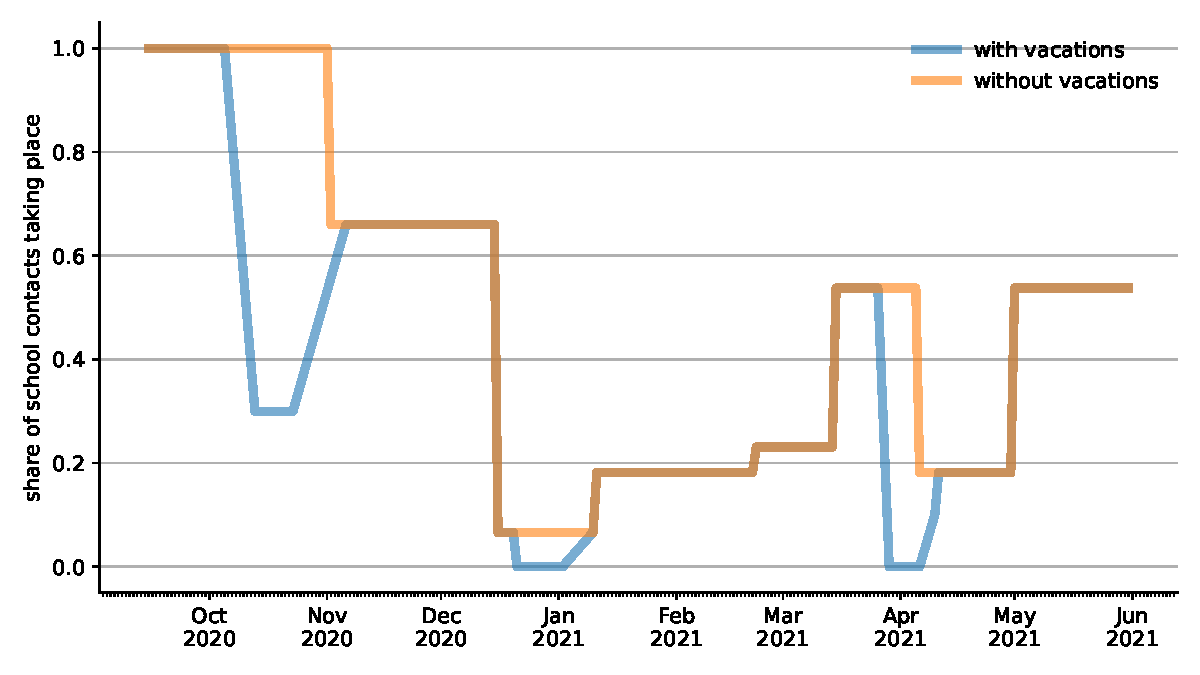
\includegraphics[width=\textwidth]{figures/results/figures/data/school_multiplier_comparison}
    \caption{School Multiplier With and Without Vacations Factored In}
    \floatfoot{\noindent \textit{Note:} The dates on which schools have vacation are
    decided at the federal level. Vacations are directly implemented in our model with no
    school contacts taking place on weekends and during vacations (by federal state) just
    like the schooling mode (full operation, emergency care, rotating schemes with half
    class sizes etc.). The figure is thus only an illustration that roughly shows the
    share of contacts taking place compared to pre-pandemic level with and without
    vacations. The difference between the lines show when vacations take place and to
    what degree. For example all states have fall vacations but the timing varies
    strongly between states.}
    \label{fig:school_multiplier}
\end{figure}


%
% Schließung von Kindertagesstätten und Schulen: 37,4 Millionen ausgefallene Arbeitstage
% http://www.iab-forum.de/schul-und-kitaschliessungen-krankheit-quarantaene-die-coronabedingten-arbeitsausfaelle-der-erwerbstaetigen-steigen-auf-592-millionen-arbeitstage/
%
%
% https://www.sueddeutsche.de/politik/schulschliessung-lockdown-bildung-1.5190377: In
% allen Ländern geht trotz des Lockdowns ein erheblicher Anteil der Schülerinnen und
% Schüler in die Schule.
% https://gfx.sueddeutsche.de/apps/e525337/www/_image_desktopw1840q70-1e2e2bf78b7d4430
% 18% der Grundschüler in Notbetreuung in BW
%

% work
For our work contacts we use the reductions in work mobility reported in the Google
Mobility Data \citep{Google2021} to calibrate our work policies. Reductions in work
contacts are not random but governed through a work contact priority where the policy
changes the threshold below which workers stay home. Figure \ref{fig:work_multiplier}
shows the share of workers that go to work in our model over time.

\begin{figure}[ht]
    \centering
    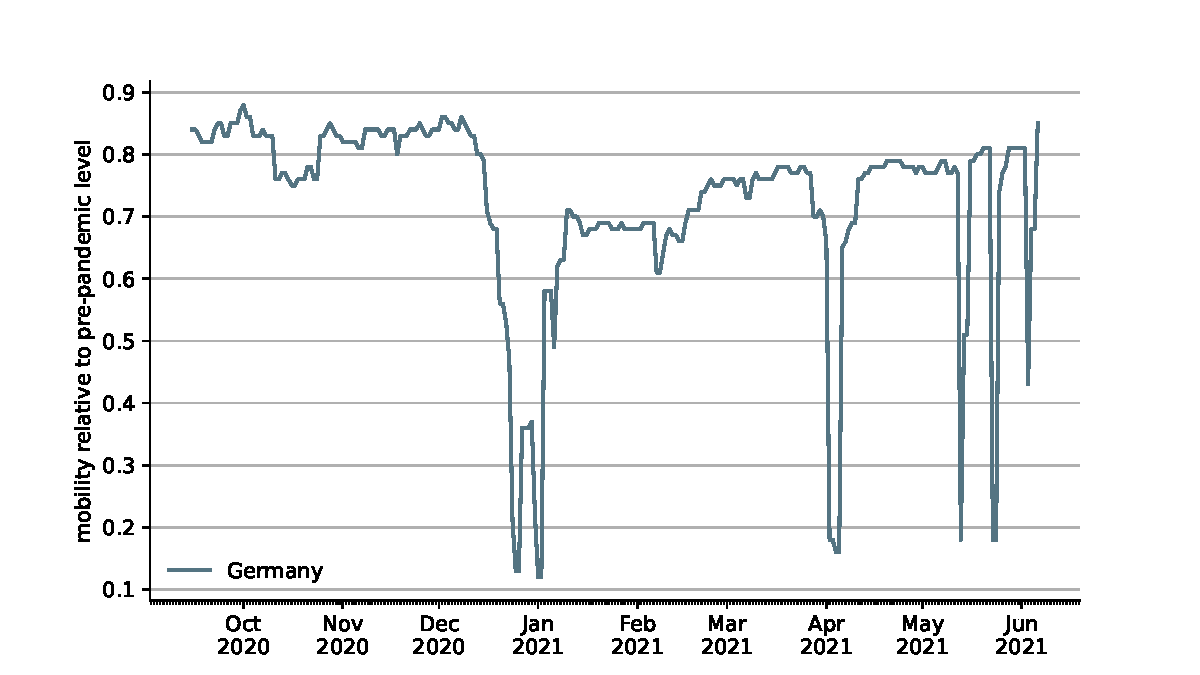
\includegraphics[width=\textwidth]{figures/results/figures/data/work_multiplier_since_sep}
    \caption{Share of Workers with Work Contacts}
    \label{fig:work_multiplier}
    \floatfoot{\noindent \textit{Note:} The figure shows the work mobility as reported by
        \cite{Google2021}. We take this as a proxy of the share of workers who are not in
        home office, i.e. who still have physical work contacts. The figure interpolates
        over weekends as we handle weekend effects through information on work on
        weekends in the German census data we use. The figure shows the share aggregated
        over Germany as a whole. To capture the effect that local policies, school
        vacations and public policies have on work contacts we use the data on the level
        of the federal states to determine which workers go to work depending on the
        state they live in.}
\end{figure}

For both work and school contacts we assume that starting November with the lockdown
light in Germany, hygiene measures (such as masks, ventilation and hand washing) became
more strict and more conscientiously observed, leading to a reduction of 33\% in the
number of contacts with the potential to transmit Covid-19.

For the last group of contacts, which cover things like leisure activities, grocery
shopping, etc., we have no reliable data by how much policies reduce them. In addition,
they are likely to be affected by social and psychological factors such as pandemic
fatigue and vacations. Because of this we estimate them like the infection probabilities
to fit the time series data. We use very few change points and tie them to particular
events such as policy announcements or particular holidays. Because of the scarce data
situation we cannot distinguish between a hygiene factor (such as mask wearing) during
meetings and physical distancing (such as virtual meetings with
friends).\comment[id=K]{@Janos: Maybe make more concrete when the estimation is finished
which phases we have and why the switching points are where they are.}

\begin{figure}
    \centering
    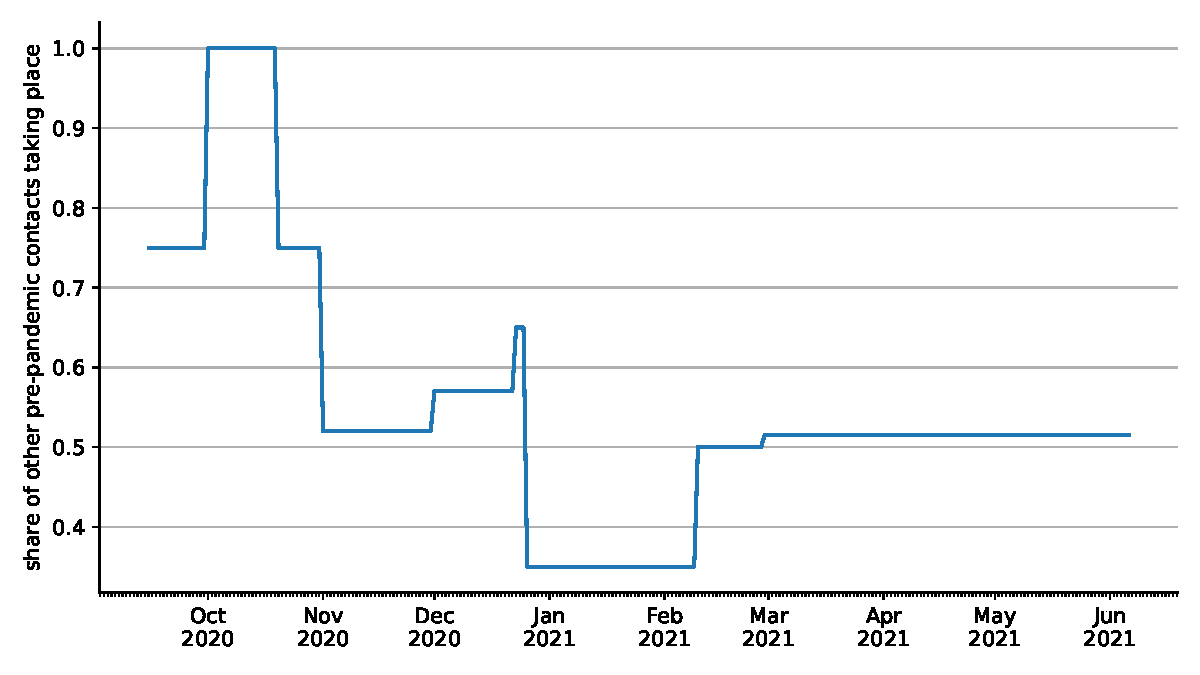
\includegraphics[width=\textwidth]{figures/results/figures/data/other_multiplier}
    \caption{Share of Pre-Pandemic Other Contacts Taking Place with Infection Potential}
    \label{fig:other_multiplier}
    \floatfoot{\noindent \textit{Note:} All values are estimated. We try to use as little
    switching points as possible and tie them to political events (such as lockdown
    announcements) unless changes are used to capture anticipation or pandemic fatigue
    (for example we model an anticipation of the November lockdown and model lockdown
    fatigue in early March).}
\end{figure}

\FloatBarrier


In our model, there are five reasons why rapid tests are done:\comment[id=J]{Add a
section on how we calibrate rapid test demand; Mainly describe the datapoints we have and
say that we usually interpolate linearly in between data points. (Only exception to that
is private rapid test demand, which we fit to data)}

\begin{enumerate}
    \item someone plans to have work contacts
    \item someone is an employee of an educational facility or a school pupil
    \item a household member has tested positive or developed symptoms
    \item someone has developed symptoms but has not received a PCR test
    \item someone plans to participate in a weekly non-work meeting
\end{enumerate}

\subsubsection{work rapid tests}

For work contacts, we know from the COSMO study (\cite{Betsch2021}, 20th/21st of April)
that 60\% of workers who receive a test offer by their employer regularly use it. We
assume this share to be time constant.

In addition, there are some surveys that allow us to trace the expansion of employers who
offer tests to their employees. Mid march, 20\% of employers offered tests to their
employees \citep{DIHK2021}. In the second half of March, 23\% of employees reported being
offered weekly rapid tests by their employer \citep{Ahlers2021}. This share increased to
60\% until the first days of April \cite{ZDF2021}.

\textcolor{red}{ToDo: Find the survey that the ZDF is citing here}

Until mid April 70\% of workers were expected to receive a
weekly test offer \citep{AerzteZeitung2021}. However, according to surveys conducted in
mid April \citep{Betsch2021}, less than two thirds of individuals with work contacts
receive a test offer. Starting on April 19th employers were required by law to provide
two weekly tests to their employees \citep{Bundesanzeiger2021}. We assume that compliance
is incomplete and only 80\% of employers actually offer tests.

\subsubsection{educ rapid tests}

We assume that employees in educational facilities start getting tested in 2021 and that
by March 1st 30\% of them are tested weekly. The share increases to 90\% for the week
before Easter. At that time both Bavaria \citep{BayrischerRundfunk2021} and
Baden-Württemberg \citep{MinisteriumKultus2021} were offering tests to teachers and
North-Rhine
Westphalia\footnote{\url{https://www.land.nrw/de/pressemitteilung/umfassende-informationen-fuer-die-schulen-zu-corona-selbsttests-fuer-schuelerinnen}}
\cite{DPA2021} and Lower Saxony \citep{SueddeutscheZeitung2021} were already testing
students and tests for students and teachers were already mandatory in Saxony
\citep{SueddeutscheZeitung2021a}. After Easter we assume that 95\% of teachers get tested
twice per week.

Tests for students started
later\footnote{\url{https://www.land.nrw/de/pressemitteilung/umfassende-informationen-fuer-die-schulen-zu-corona-selbsttests-fuer-schuelerinnen}}
\citep{MinisteriumKultus2021} so we assume that they only start in February and only 10\%
of students get tested by March 1st. Relying on the same sources as above we approximate
that by the week before Easter this share had increased to 40\%.\footnote{\url{https://www.land.nrw/de/pressemitteilung/umfassende-informationen-fuer-die-schulen-zu-corona-selbsttests-fuer-schuelerinnen}, }

After Easter the share of students receiving twice weekly tests is set to 75\%. This as
based on tests becoming mandatory becoming mandatory in Bavaria after Easter
break\footnote{Bavaria\footnote{\url{https://bit.ly/3nz5fXS}}, in North-Rhine Westphalia
on April
12th\footnote{https://www.schulministerium.nrw/ministerium/schulverwaltung/schulmail-archiv/14042021-schulbetrieb-im-wechselunterricht-ab-montag},
\url{https://bit.ly/2QHilX3}} and on the 19th in
Baden-Württemberg\footnote{https://bit.ly/3vuetaD, https://bit.ly/3vuetaD}.


To limit our degrees of freedom, we only have one parameter that governs how many
individuals do a rapid test because of any of the private demand reasons (own symptoms
but no PCR test, planned weekly leisure meeting or a symptomatic or positively tested
household member).

We assume that there is no private rapid test demand until March when both the citizens'
tests and rapid tests for lay people started to become available
\footnote{\url{https://bit.ly/3ehmGcj}, \url{https://bit.ly/3xJCIn8}} and other access to
rapid tests was very limited.

According to the COSMO study\footnote{\url{https://bit.ly/2QSFAgR}} 63\% would have been
willing to take a test in the round of 23rd of February 2021 when an acquaintance would
have tested positive. Since this is only asking for willingness not actual behavior and
the demand when meeting with friends is very likely lower, we take this as the upper
bound of private rapid test demand which is reached on May 4th. To cover that many people
are likely to have sought and done their first rapid test before the Easter holidays to
meet friends or family, we let the share of individuals doing rapid tests in that time
increase more rapidly than before and after. By end of March 25\% of individuals would do
a rapid test due to a private reason.



All shares of individuals who would take a rapid test if the conditions were met can be
seen in Figure~\ref{fig:rapid_test_demand}.

\begin{figure}
    \centering
    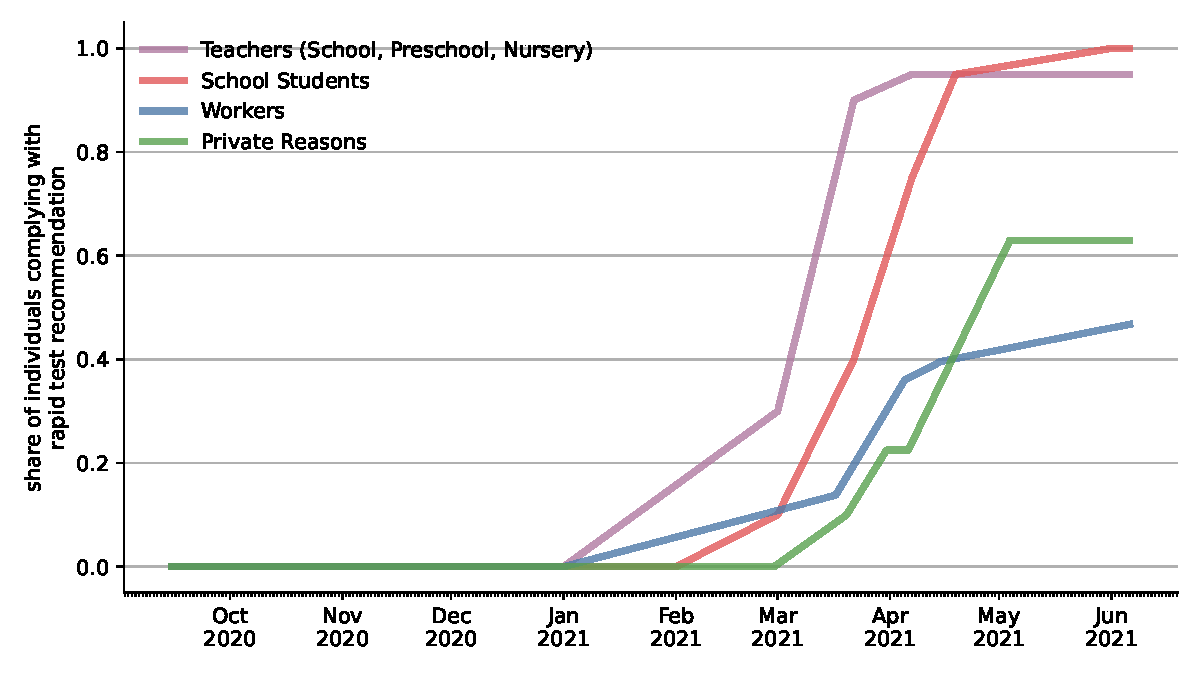
\includegraphics[width=\textwidth]{figures/results/figures/data/testing/rapid_test_demand_shares}
    \caption{\textbf{Share of Individuals Doing a Rapid Test.}}
    \floatfoot{\noindent \textit{Note:} Rapid test demand can be triggered by individuals
    planning to have education contacts, work contacts, developing symptoms without
    access to a PCR test, having a household member with a positive test or symptoms. In
    each case whether a rapid test is done depends on how long it has been since the
    individual's last rapid test and her individual compliance parameters. As an example,
    take a worker in May. In that time workers are encouraged to test themselves twice
    weekly but there is no general requirement to test themselves. If the worker has not
    done a test within the last four days in our model she will demand a test if her
    (time-constant) compliance parameter belongs to the upper 60\% in the population.}
    \label{fig:rapid_test_demand}
\end{figure}


\begin{figure}[ht]
    \centering
    \caption{Share of Individuals With Rapid Tests}
    \label{fig:share_ever_rapid_test}
    \begin{subfigure}{.55\textwidth}
        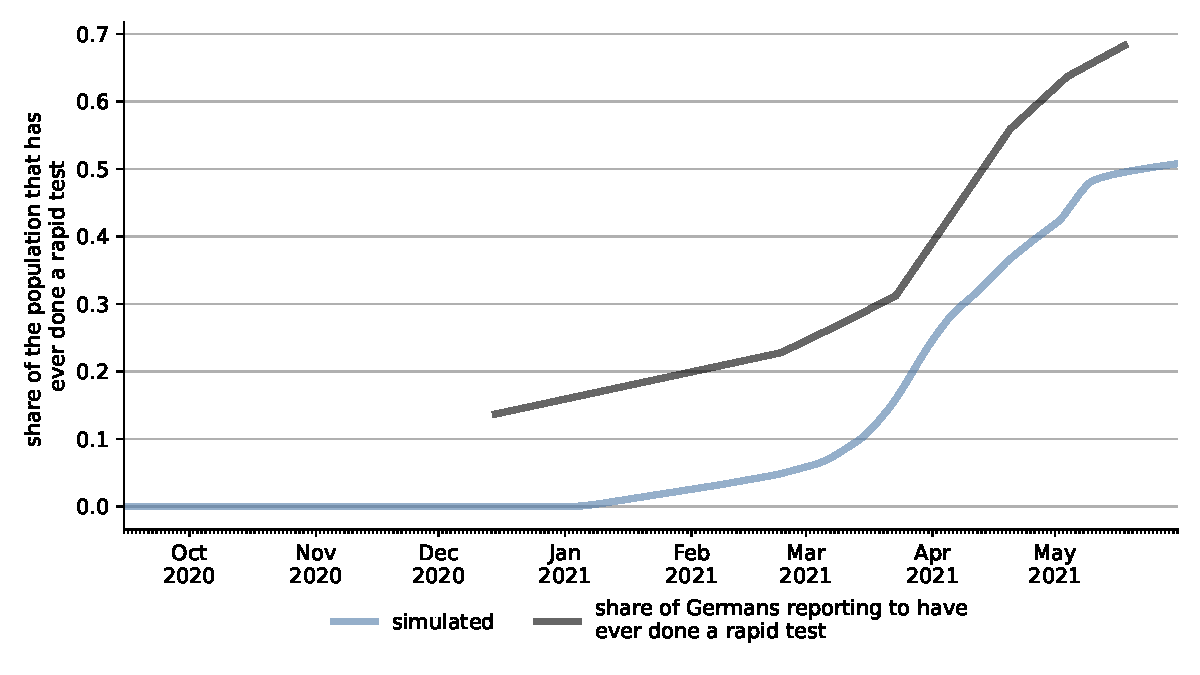
\includegraphics[width=0.9 \textwidth]{figures/results/figures/scenario_comparisons/combined_fit/full_share_ever_rapid_test}
        \caption{Share of Individuals That Have Ever Done a Rapid Test}
    \end{subfigure}%
    \begin{subfigure}{.55\textwidth}
        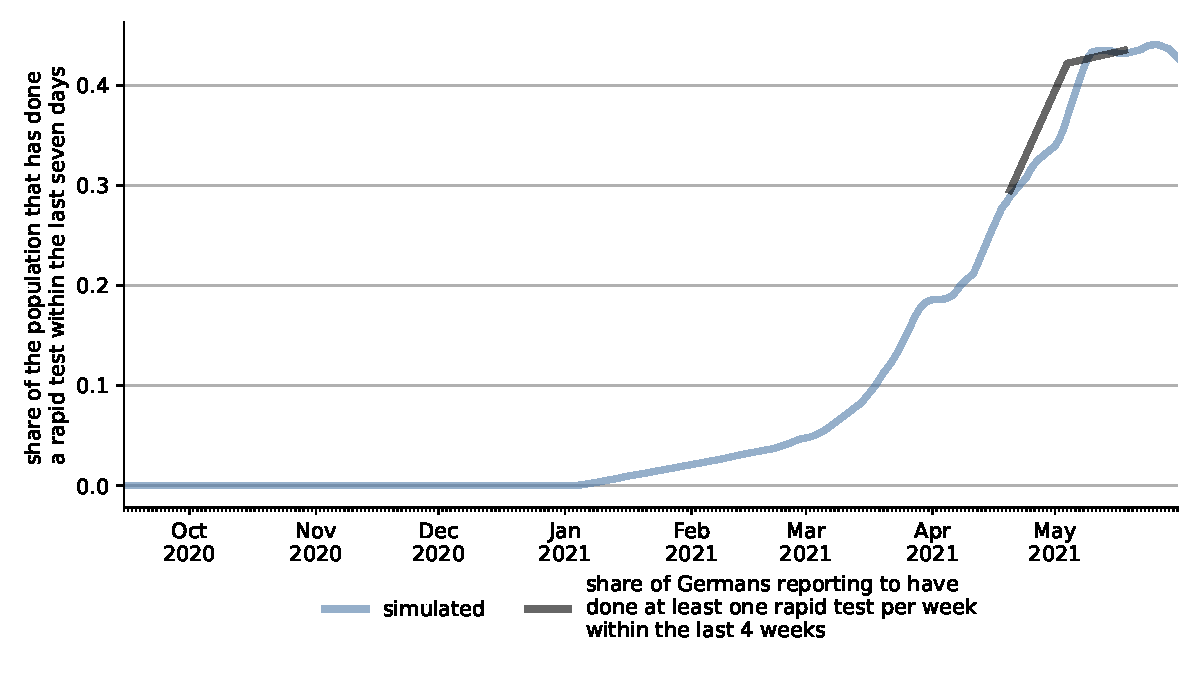
\includegraphics[width=0.9 \textwidth]{figures/results/figures/scenario_comparisons/combined_fit/full_share_rapid_test_in_last_week}
        \caption{Share of Individuals Having Done a Rapid Test in the Last Week}
    \end{subfigure}
    \label{fig:share_rapid_test_last_week}
    \floatfoot{\noindent \textit{Note:} The figure compares the share of individuals who
        have ever done a rapid test or done a rapid test within the last week in our
        simulations to the shares reported in the
        \href{https://projekte.uni-erfurt.de/cosmo2020/web/topic/wissen-verhalten/80-schnelltests/}{COVID-19
        Snapshot Monitoring Survey}. The left panel compares the share of individuals who
        have ever done a rapid test. The right panel compares the share of individuals
        who have done a rapid test within the last seven days in our simulation compared
        to the share reporting to have done at least weekly rapid tests in the last four
        weeks in the COSMO survey. Overall our calibration of rapid tests are slightly
        conservative. The overall share is below that in the study. We fit the share of
        weekly tests quite exactly. However, the study only covers adults while our share
        also includes children who are tested very regularly when attending school.}
\end{figure}

 \comment[id=K]{J: Explain that we don't fit the share ever tested that well because our rapid test compliance is completely fixed. }

\FloatBarrier